\documentclass[notes,blackandwhite,mathsans,usenames,dvipsnames]{beamer}

\usepackage{amsmath}
\usepackage{amssymb}
\usepackage{graphicx}
\usepackage{fancybox}
\usepackage{booktabs}
\usepackage{multirow,pxfonts}
\usepackage{cmbright}
\usepackage{xcolor}
\usepackage{color}
\usepackage{enumitem}
\usepackage{animate}
\usepackage{changepage}
\usepackage{multicol}

\usepackage[T1]{fontenc}
\fontencoding{T1}  
\usepackage[utf8]{inputenc}


\usefonttheme{default}
\setbeamercovered{invisible}
\beamertemplatenavigationsymbolsempty

\makeatletter
\setbeamertemplate{footline}
{
  \leavevmode
  \hbox{
  \begin{beamercolorbox}[wd=0.97\paperwidth,ht=2.25ex,dp=2ex,right]{}
{\color{mcxs2} \insertframenumber{} }
  \end{beamercolorbox}}%
}


\definecolor{mcxs1}{HTML}{05386B}
\definecolor{mcxs2}{HTML}{379683}
\definecolor{mcxs3}{HTML}{5CDB95}
\definecolor{mcxs4}{HTML}{8EE4AF}
\definecolor{mcxs5}{HTML}{EDF5E1}
\setbeamercolor{frametitle}{fg=mcxs2}
\AtBeginDocument{\color{mcxs1}}
\setbeamertemplate{itemize item}[triangle]


\begin{document}

%\fontfamily{pag}\selectfont
%\setbeamerfont{title}{family=\fontfamily{pag}\selectfont}
%\setbeamerfont{frametitle}{family=\fontfamily{pag}\selectfont}
%\setbeamerfont{framesubtitle}{family=\fontfamily{pag}\selectfont}







{\setbeamercolor{background canvas}{bg=mcxs4}
\begin{frame}
\centering
\vspace{1cm}\textbf{\Large\color{mcxs2} Macroeconometrics}

\vspace{1cm}{\Large \textbf{Lecture 20 {\color{purple} Stochastic Volatility models}}}

\vspace{1cm}\textbf{Tomasz Wo\'zniak}

\vspace{0.3cm}{\small\color{mcxs2} Department of Economics\\ University of Melbourne}

\end{frame}





\begin{frame}

\vspace{1cm}\textbf{\color{mcxs2}A simple Stochastic Volatility model}

%\bigskip\textbf{\color{mcxs2}Log-normal distribution}

\bigskip\textbf{\color{purple}Unconditional moments}

\bigskip\textbf{\color{mcxs2}Conditional heteroskedasticity of the All Ordinaries Index}

%\bigskip\textbf{\color{mcxs2}Heteroskedastic trend or heteroskedastic cycle?}


%\small
%\vspace{1cm} Compulsory readings: \scriptsize
%
%\smallskip{\color{mcxs2}Wo\'zniak (2019) Bayesian Structural VARs: Algorithms and Inference, Lecture notes}


\vspace{1cm} References: \footnotesize

\smallskip{\color{mcxs2}Jacquier, Polson, Rossi (1994) Bayesian Analysis of Stochastic Volatility Models, Appendix A, Journal of Business \& Economic Statistics}


\normalsize
\bigskip Materials: \scriptsize

\smallskip{\color{mcxs2}A zip file} \texttt{L20 mcxs.zip} {\color{mcxs2}for the reproduction of the results}

\end{frame}




\begin{frame}{Stochastic Volatility models}

\begin{description}
\item[Stochastic Volatility models] {\color{mcxs2}provide a flexible way of modeling and forecasting conditional variances of time series}

\bigskip\item[Estimation of SV models] {\color{mcxs2}for heteroskedastic data improved precision of the estimation}

\bigskip\item[Many recent empirical studies] {\color{mcxs2}provide evidence that conditional heteroskedasticity modelled with SV process is the most important extension of macroeconomic models} {\color{purple}improving the forecast precision to a largest extent}

\bigskip\item[Bayesian estimation] {\color{mcxs2}via the Gibbs sampler using the simulation smoother and an} {\color{purple}auxiliary mixture} {\color{mcxs2}is efficient and computationally fast}
\end{description}
\end{frame}





\begin{frame}

\bigskip\textbf{\color{mcxs1}Objectives.}
\begin{itemize}[label=$\blacktriangleright$]
\item {\color{mcxs1}To introduce a basic model for conditional heteroskedasticity}
\item {\color{mcxs1}To investigate the properties of the data that the model can capture}
\item {\color{mcxs1}To familiarise with the estimation outcomes and basic interpretations}
\end{itemize}

\bigskip\textbf{\color{purple}Learning outcomes.}
\begin{itemize}[label=$\blacktriangleright$]
\item {\color{purple}Specifying stationary and non-stationary volatility processes}
\item {\color{purple}Understanding of the benefits of modeling heteroskedasticity}
\item {\color{purple}Analysing a log-normally distributed random process}
\end{itemize}

\end{frame}







\begin{frame}

\begin{adjustwidth}{-0.5cm}{0cm}
\vspace{8.3cm}\Large
\textbf{{\color{mcxs2}A simple} {\color{purple}Stochastic Volatility} {\color{mcxs2} model}}
\end{adjustwidth}

\end{frame}
}


\begin{frame}{A simple Stochastic Volatility model}

\begin{align*}
y_t &= \sqrt{h_t} \epsilon_t\\[1ex]
\log h_t &= \mu_0 + \alpha\log h_{t-1} + \sigma_v v_t\\[1ex]
\epsilon_t &\sim\mathcal{N}(0,1)\\[1ex]
v_t &\sim\mathcal{N}(0,1)
\end{align*}

\begin{description}
\item[$y_t$] {\color{mcxs2}-- a zero mean real-valued random variable}
\item[$h_t$] {\color{mcxs2}-- a conditional variance of} $y_t$
\item[$\log h_t$] {\color{mcxs2}-- log of conditional variance of} $y_t$
\item[$\mu_0$], $\alpha$, $\sigma_v$ {\color{mcxs2}-- parameters of the model}
\item[$\epsilon_t, v_t$] {\color{mcxs2}-- error terms of the measurement and state equation respectively}
\end{description}
\end{frame}




\begin{frame}{A simple Stochastic Volatility model}

\textbf{Predictive density of} $\log h_t$
\begin{align*}
\log h_t &= \mu_0 + \alpha\log h_{t-1} + \sigma_v v_t\\
v_t &\sim\mathcal{N}(0,1)\\
\downarrow&\\
\log h_t|\log h_{t-1}, \mu_0, \alpha, \sigma_v &\sim\mathcal{N}(\mu_0 + \alpha\log h_{t-1}, \sigma_v^2)
\end{align*}

\end{frame}




\begin{frame}{A simple Stochastic Volatility model}

\textbf{Unconditional moments of} $\log h_t$
\begin{align*}
\mathbb{E}[\log h_t] &= \mathbb{E}[\mu_0 + \alpha\log h_{t-1} + \sigma_v v_t]\\
&= \mu_0 + \alpha\mathbb{E}[\log h_{t-1}] + \sigma_v \mathbb{E}[v_t]\\
&= \mu_0 + \alpha\mathbb{E}[\log h_{t-1}] \\[2ex]
\text{\color{mcxs2}Assume stationarity: } & |\alpha|<1\text{\color{mcxs2}, and }\mathbb{E}[\log h_{t}]=\mathbb{E}[\log h_{t-1}]\\[2ex]
(1-\alpha)\mathbb{E}[\log h_t]&= \mu_0 \\
\mathbb{E}[\log h_t]&= \frac{\mu_0 }{1-\alpha}
\end{align*}

\end{frame}



\begin{frame}{A simple Stochastic Volatility model}

\textbf{Unconditional moments of} $\log h_t$
\begin{align*}
\mathbb{V}ar[\log h_t] &= \mathbb{V}ar[\mu_0 + \alpha\log h_{t-1} + \sigma_v v_t]\\
&= \alpha^2\mathbb{V}ar[\log h_{t-1}] + \sigma_v^2 \mathbb{V}ar[v_t]\\
&= \alpha^2\mathbb{V}ar[\log h_{t-1}] + \sigma_v^2 1\\[2ex]
\text{\color{mcxs2}Assume stationarity } & |\alpha|<1\text{\color{mcxs2}, and }\mathbb{V}ar[\log h_{t}]=\mathbb{V}ar[\log h_{t-1}]\\[2ex]
(1-\alpha^2)\mathbb{V}ar[\log h_t]&= \sigma_v^2 \\
\mathbb{V}ar[\log h_t]&= \frac{\sigma_v^2 }{1-\alpha^2}
\end{align*}

\end{frame}



\begin{frame}{A simple Stochastic Volatility model}

\textbf{Unconditional distribution of} $\log h_t$
\begin{align*}
\log h_t &\sim\mathcal{N}\left(\frac{\mu_0 }{1-\alpha},   \frac{\sigma_v^2 }{1-\alpha^2}\right)
\end{align*}

\bigskip\textbf{Unconditional distribution of} $h_t$
\begin{align*}
h_t &\sim\log\mathcal{N}\left(\frac{\mu_0 }{1-\alpha},   \frac{\sigma_v^2 }{1-\alpha^2}\right)
\end{align*}

\end{frame}



{\setbeamercolor{background canvas}{bg=mcxs4}
\begin{frame}

\begin{adjustwidth}{-0.5cm}{0cm}
\vspace{8.3cm}\Large
\textbf{{\color{mcxs2}Unconditional} {\color{purple}moments} }
\end{adjustwidth}

\end{frame}
}



\begin{frame}{Log-normal distribution}

\bigskip {\color{mcxs2}Let} $x$ {\color{mcxs2}be a positive real-valued random variable the log of which is normally distributed.} {\color{mcxs2}Then,} $x$ {\color{mcxs2}is} {\color{purple}log-normally distributed}.
\begin{align*}
\log x &\sim\mathcal{N}\left(\mu, \sigma^2\right)\\[1ex]
x &\sim\log\mathcal{N}\left(\mu, \sigma^2\right)
\end{align*}
\begin{description}
\item[$\mu$] {\color{mcxs2}-- a mean parameter of the log-normal distribution}
\item[$\sigma^2$] {\color{mcxs2}-- a variance parameter of the log-normal distribution}
\item[$\frac{1}{x}$] {\color{mcxs2}-- the Jacobian of the transformation}
\end{description}

\bigskip\textbf{Density function.}
\begin{align*}
\frac{1}{\sqrt{2\pi\sigma^2}}\frac{1}{x}\exp\left\{ -\frac{1}{2}\frac{(\log x - \mu)^2}{\sigma^2} \right\}
\end{align*}
\textbf{Moments.} {\color{mcxs2}All of the moments exist and can be computed using:}
$$ \mathbb{E}[x^n]=\exp\left\{ n\mu+\frac{n^2\sigma^2}{2} \right\} $$

\end{frame}




\begin{frame}{Unconditional moments}

\textbf{Unconditional moments of} $y_t$
\begin{align*}
\mathbb{E}[y_t] &= \mathbb{E}\left[\sqrt{h_t}\epsilon_t\right]\overset{LIE}{=}\mathbb{E}\left[\sqrt{h_t}\mathbb{E}_{t-1}[\epsilon_t]\right] = 0\\[2ex]
\mathbb{E}\left[y_t^2\right] &= \mathbb{E}\left[h_t\epsilon_t^2\right]= \mathbb{E}\left[h_t\right]\mathbb{E}\left[\epsilon_t^2\right]= \mathbb{E}\left[h_t\right]1\\
&= \exp\left\{ \frac{\mu_0 }{1-\alpha} + \frac{\sigma_v^2 }{2\left(1-\alpha^2\right)} \right\} \\[2ex]
\mathbb{E}\left[y_t^3\right] &= \mathbb{E}\left[h_t^{\frac{3}{2}}\epsilon_t^3\right]=  \mathbb{E}\left[h_t^{\frac{3}{2}}\right]\mathbb{E}\left[\epsilon_t^3\right] = 0\\[2ex]
\mathbb{E}\left[y_t^4\right] &= \mathbb{E}\left[h_t^{2}\epsilon_t^4\right]=  3\mathbb{E}\left[h_t^2\right]\\
&= 3\exp\left\{ \frac{2\mu_0 }{1-\alpha}+ \frac{2\sigma_v^2 }{1-\alpha^2}\right\}
\end{align*}

\end{frame}




\begin{frame}{Unconditional moments}

\textbf{Unconditional moments of} $y_t$
\begin{align*}
Kurtosis[y_t]&= \frac{\mathbb{E}\left[y_t^4\right]}{\mathbb{E}\left[y_t^2\right]^2}= \frac{3\exp\left\{ \frac{2\mu_0 }{1-\alpha}+ \frac{2\sigma_v^2 }{1-\alpha^2}\right\}}{\exp\left\{ \frac{2\mu_0 }{1-\alpha} + \frac{2\sigma_v^2 }{2\left(1-\alpha^2\right)} \right\}}\\
&=3\exp\left\{ \frac{\sigma_v^2 }{1-\alpha^2}\right\}>3\\[2ex]
\mathbb{E}\left[ y_t^2y_{t-s}^2 \right] &= \mathbb{E}\left[ h_t h_{t-s} \right]= \exp\left\{ \frac{2\mu_0 }{1-\alpha} + \frac{(1-\alpha^s)\sigma_v^2 }{1-\alpha^2} \right\}
\end{align*}\footnotesize

\bigskip{\color{mcxs2}For the derivation see Jacquier, Polson, Rossi (1994, JBES, Appendix A)}
\end{frame}




\begin{frame}{A simple Stochastic Volatility model}
\textbf{An alternative notation.	}
\begin{align*}
y_t &= \exp\left\{\frac{1}{2}h_t\right\} \epsilon_t\\[1ex]
h_t &= \mu_0 + \alpha h_{t-1} + \sigma_v v_t\\[1ex]
\epsilon_t &\sim\mathcal{N}(0,1)\\[1ex]
v_t &\sim\mathcal{N}(0,1)
\end{align*}

\bigskip\begin{description}
\item[$h_t$] {\color{mcxs2}-- log of conditional variance of} $y_t$
\item[$\sigma_{y.t}^2 = \exp\left\{h_t\right\}$] {\color{mcxs2}-- a conditional variance of} $y_t$
\end{description}
\end{frame}





{\setbeamercolor{background canvas}{bg=mcxs4}
\begin{frame}


\begin{adjustwidth}{-0.5cm}{0cm}
\vspace{7.8cm}\Large
\textbf{{\color{mcxs2}Conditional heteroskedasticity}\\ {\color{purple}of the All Ordinaries Index} }
\end{adjustwidth}

\end{frame}
}





\begin{frame}{Conditional heteroskedasticity of the All Ordinaries Index}
\begin{center}
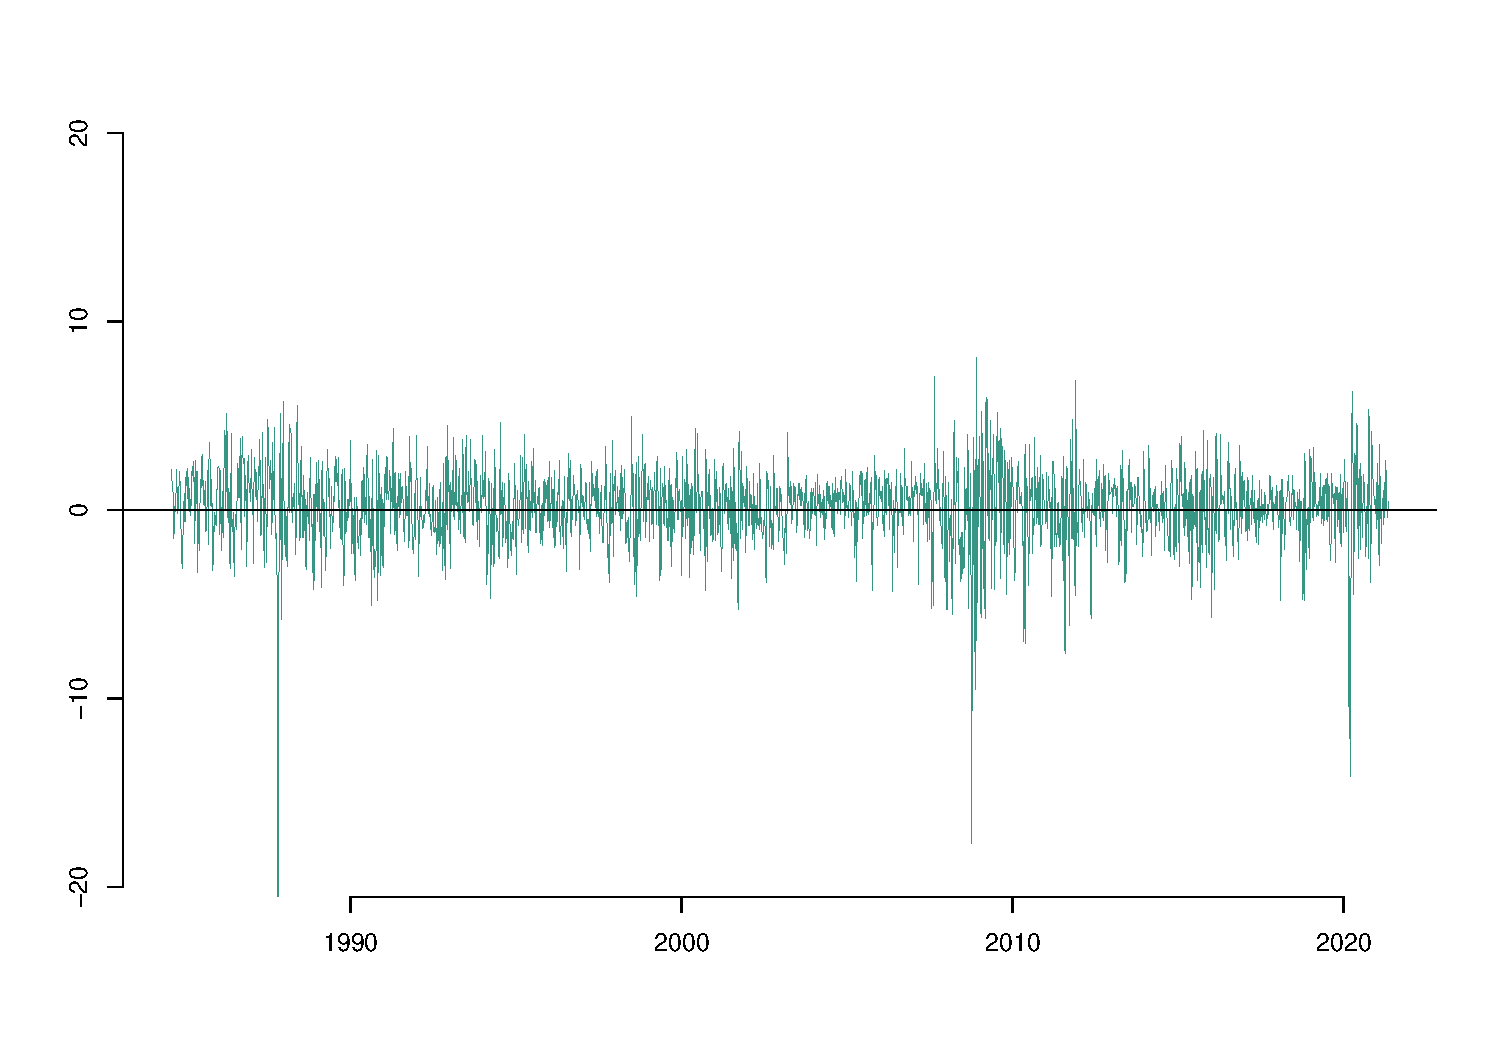
\includegraphics[scale=0.48, trim=1.5cm 2cm 0cm 3.1cm]{aord.pdf}

\bigskip\small{\color{mcxs2}Weekly log-returns in pp. from August 1984 to May 2021\\ Source: Yahoo Finance ($T=1919$)\\

\smallskip The series clearly exhibits volatility clustering}
\end{center}
\end{frame}




\begin{frame}{Conditional heteroskedasticity of the All Ordinaries Index}
\begin{center}
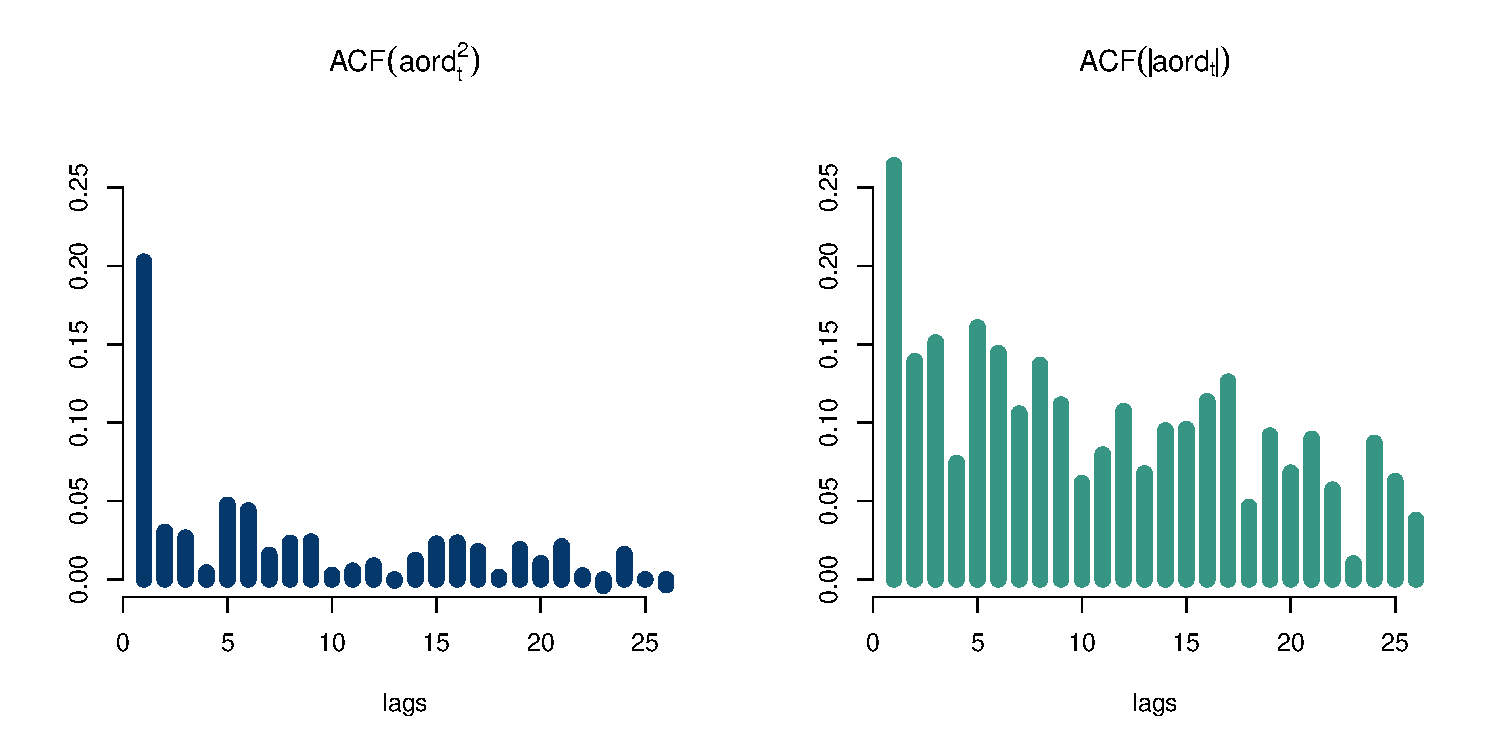
\includegraphics[scale=0.48, trim=1.5cm 0cm 0cm 1cm]{aord-acf.pdf}

\bigskip\small{\color{mcxs2}The heteroskedasticity of the data seems to be persistent}
\end{center}
\end{frame}





\begin{frame}{Conditional heteroskedasticity of the All Ordinaries Index}

\begin{multicols}{2}
\textbf{SV model.}
\begin{align*}
y_t &= \exp\left\{\frac{1}{2}h_t\right\} \epsilon_t\\[1ex]
h_t &= h_{t-1} + \sigma_v v_t\\[1ex]
\epsilon_t &\sim\mathcal{N}(0,1)\\[1ex]
v_t &\sim\mathcal{N}(0,1)
\end{align*}

\columnbreak

\textbf{SV--AR model.}
\begin{align*}
y_t &= \exp\left\{\frac{1}{2}h_t\right\} \epsilon_t\\[1ex]
h_t &= \mu_0 + \alpha h_{t-1} + \sigma_v v_t\\[1ex]
\epsilon_t &\sim\mathcal{N}(0,1)\\[1ex]
v_t &\sim\mathcal{N}(0,1)
\end{align*}

\end{multicols}


\bigskip\begin{description}
\item[$h_0$] {\color{mcxs2}-- initial condition to be estimated}
\end{description}
\end{frame}





\begin{frame}{Conditional heteroskedasticity of the All Ordinaries Index}
\begin{center}
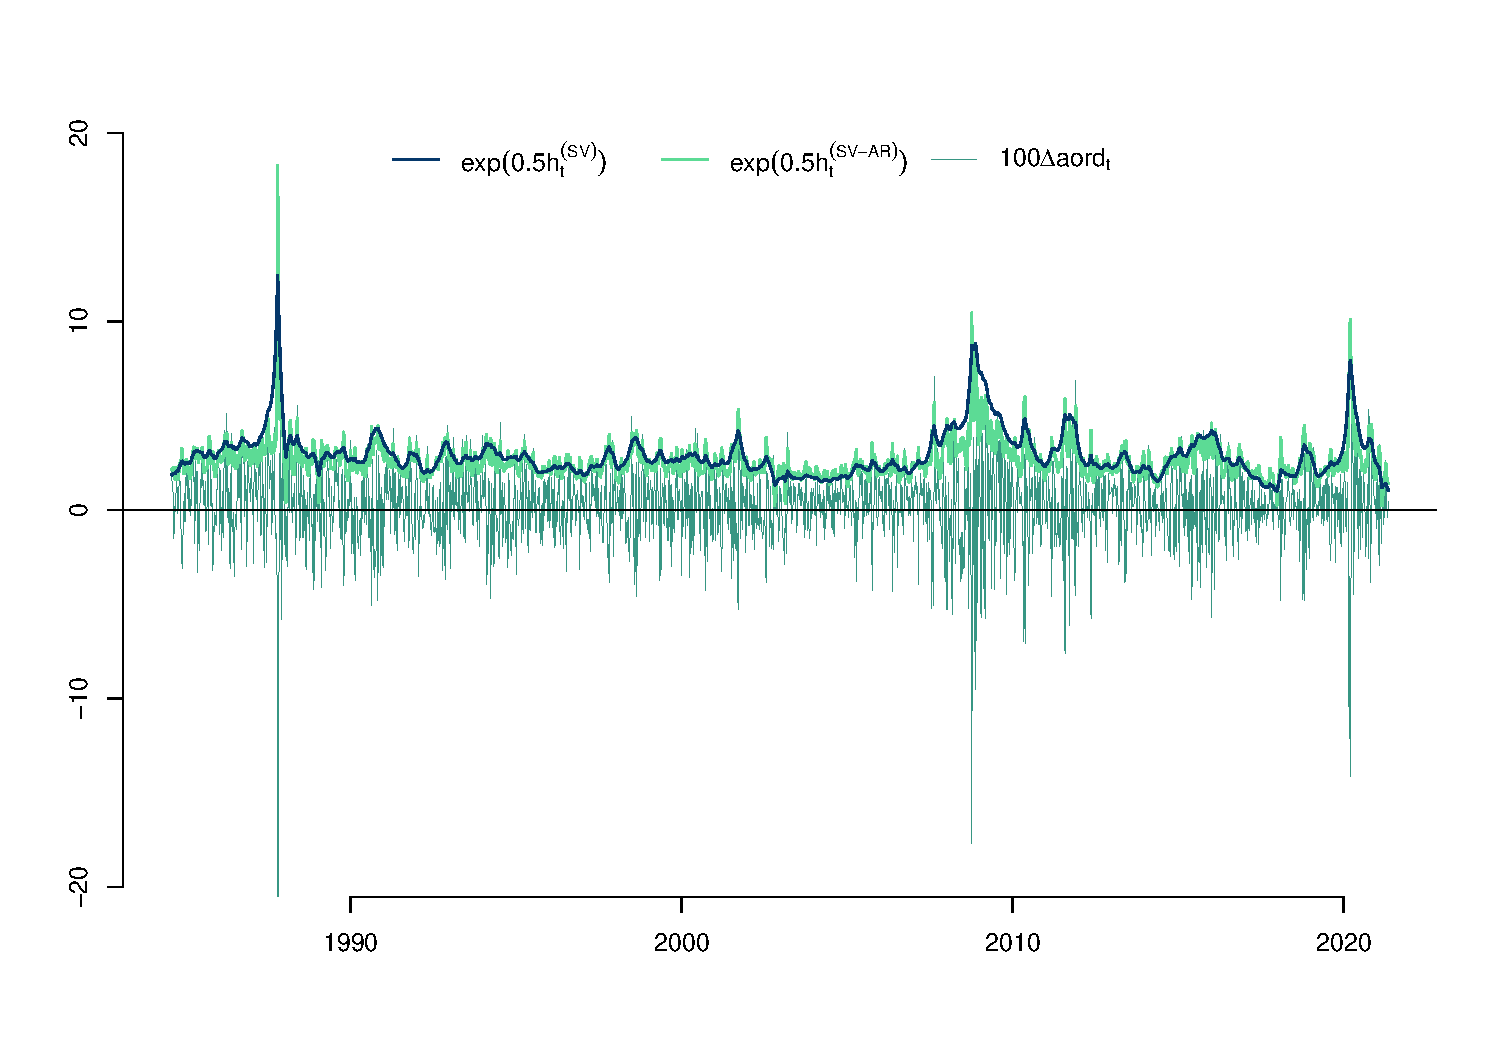
\includegraphics[scale=0.48, trim=1.5cm 2cm 0cm 3.1cm]{sv.pdf}

\bigskip\small{\color{mcxs2}The estimated conditional standard deviations capture\\ the volatility clustering accurately}
\end{center}
\end{frame}



\begin{frame}{Conditional heteroskedasticity of the All Ordinaries Index}
\begin{center}
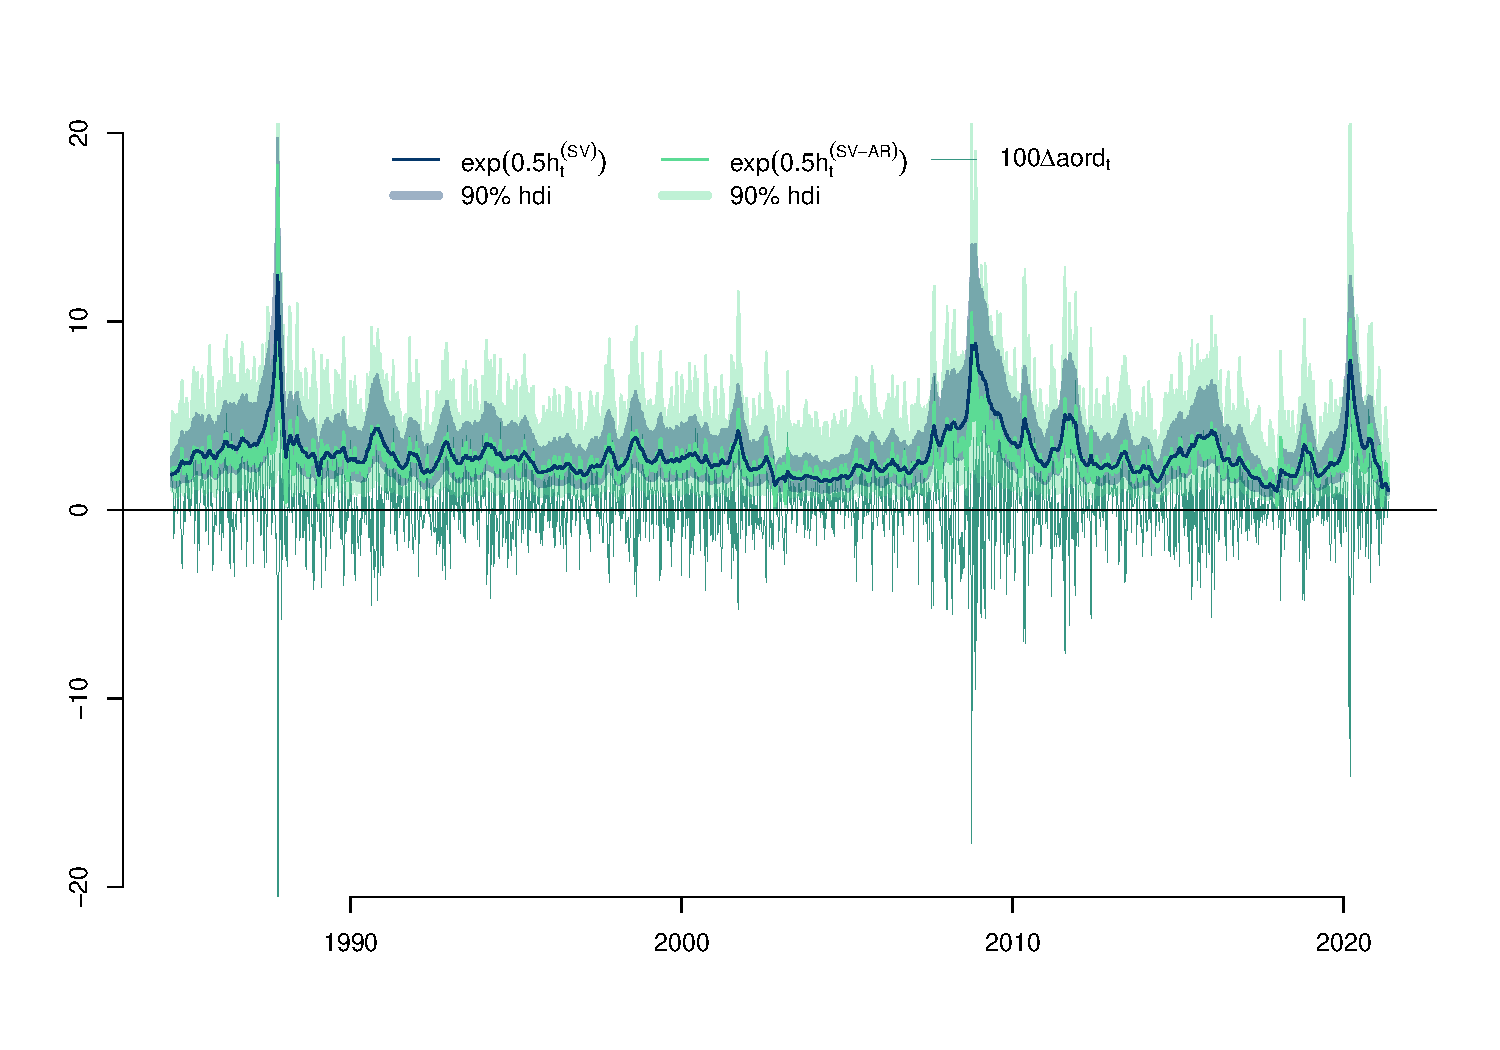
\includegraphics[scale=0.48, trim=1.5cm 2cm 0cm 3.1cm]{sv-hdi.pdf}

\bigskip\small{\color{mcxs2}Volatility estimates from the SV model seem to be more smooth\\ Volatility estimates from the SV-AR model seem to be more volitile }
\end{center}
\end{frame}



\begin{frame}{Conditional heteroskedasticity of the All Ordinaries Index}
\begin{center}
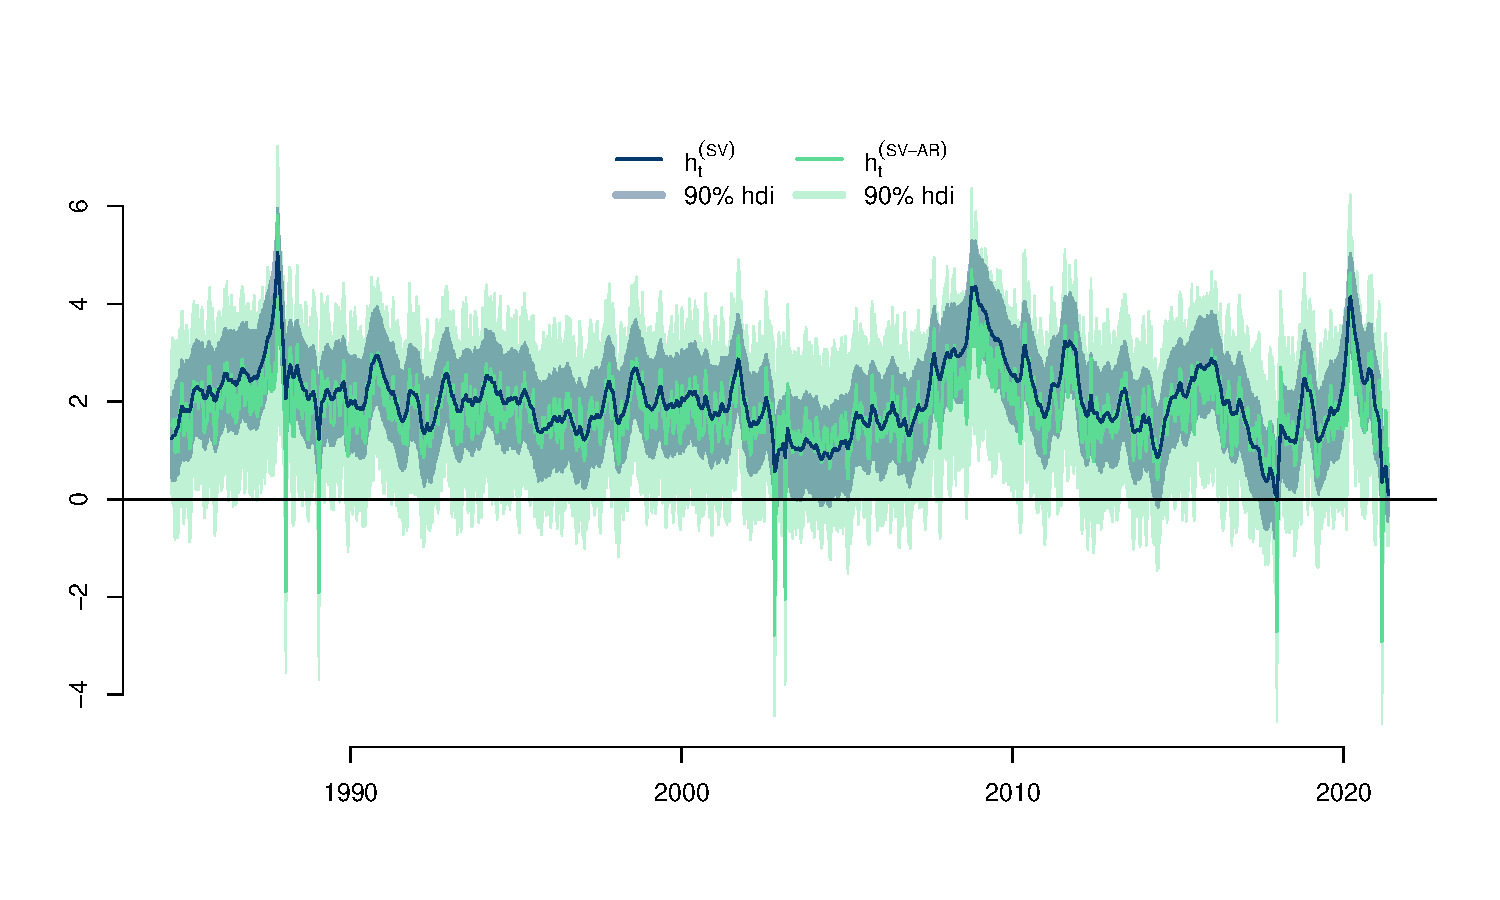
\includegraphics[scale=0.48, trim=1.5cm 1cm 0cm 3.1cm]{sv-ht.pdf}

\bigskip\small{\color{mcxs2}Volatility estimates from the SV model seem to be more smooth\\ Volatility estimates from the SV-AR model seem to be more volitile }
\end{center}
\end{frame}




\begin{frame}{Conditional heteroskedasticity of the All Ordinaries Index}
\begin{center}
\textbf{Parameter estimation results}

\bigskip
\begin{tabular}{ccccc}
\toprule
& $h_0$ & $\sigma_v^2$ & $\mu_0$ & $\alpha$\\
\midrule
SV model&1.145 & 0.092 &&\\
&(0.549) & (0.021)  &&\\[1ex]
SV--AR model&0.647 & 1.029 & 0.684 & 0.621\\
&(0.944) & (0.089) & (0.238) & (0.132) \\[1ex]
\bottomrule
\end{tabular}

\bigskip\small Posterior means and standard deviations (in parentheses) are reported
\end{center}
\end{frame}




%{\setbeamercolor{background canvas}{bg=mcxs4}
%\begin{frame}
%
%
%\begin{adjustwidth}{-0.5cm}{0cm}
%\vspace{7.8cm}\Large
%\textbf{{\color{mcxs2}Heteroskedastic trend}\\ {\color{purple}or heteroskedastic cycle?} }
%\end{adjustwidth}
%
%\end{frame}
%}
%
%
%
%\begin{frame}{Heteroskedastic trend or heteroskedastic cycle?}
%
%\textbf{Homoskedastic UC-AR(p) model.}
%\begin{align*}
%y_t &= \tau_t + \epsilon_t\\[1ex]
%\tau_t &= \mu + \tau_{t-1} + \eta_t\\[1ex]
%\epsilon_t &= \alpha_1\epsilon_{t-1} + \dots + \alpha_p\epsilon_{t-p} +  e_t \\[2ex]
%\eta_t  &\sim \mathcal{N}\left(0, \sigma_\eta^2 \right)\\
%e_t &\sim \mathcal{N}\left(0, \sigma_e^2 \right)
%\end{align*}
%
%
%\bigskip$\sigma^2_\eta / \sigma^2_e$ {\color{mcxs2}-- signal-to-noise ratio}
%
%%\bigskip{\color{mcxs2}Estimation via Gibbs sampler as presented in Lectures 18 and 19}
%
%\end{frame}
%
%
%
%\begin{frame}{Heteroskedastic trend or heteroskedastic cycle?}
%
%\centering
%\textbf{Trend inflation for Homoskedastic UC-AR(2) model.}
%\includegraphics[scale=0.45, trim=2cm 2cm 2cm 2cm ]{uc-ar2-trend.pdf}
%
%\end{frame}
%
%
%
%\begin{frame}{Heteroskedastic trend or heteroskedastic cycle?}
%
%\textbf{Heteroskedastic UC-AR(p) model.}
%\begin{align*}
%y_t &= \tau_t + \epsilon_t&&\\[1ex]
%\tau_t &= \mu + \tau_{t-1} + \eta_t & \eta_t  &\sim \mathcal{N}\left(0, \exp\left\{\frac{1}{2}h_{\eta.t}\right\} \right)\\
%\epsilon_t &= \alpha_1\epsilon_{t-1} + \dots + \alpha_p\epsilon_{t-p} +  e_t &e_t &\sim \mathcal{N}\left(0, \exp\left\{\frac{1}{2}h_{e.t}\right\} \right)\\[2ex]
%h_{\eta.t} &= h_{\eta.t-1} + v_{\eta.t}& v_{\eta.t}  &\sim \mathcal{N}\left(0, \sigma_\eta^2 \right)\\[1ex]
%h_{e.t} &= h_{e.t-1} + v_{e.t}& v_{e.t} &\sim \mathcal{N}\left(0, \sigma_e^2 \right)
%\end{align*}
%
%\small
%\bigskip{\color{mcxs2}Parameters to be estimated:}
%$\tau, \epsilon, \alpha, \beta, {\color{purple}h_\eta, h_e, h_{\eta.0}, h_{e.0}, \sigma_\eta^2}\text{, and }{\color{purple}\sigma_e^2}$
%
%\smallskip{\color{mcxs2}Derivations for} ${\color{purple}h_\eta, h_e, h_{\eta.0}, h_{e.0}, \sigma_\eta^2},{\color{purple}\sigma_e^2}$ {\color{mcxs2}will be presented during the next lecture.}
%
%\end{frame}
%
%
%\begin{frame}{Heteroskedastic trend or heteroskedastic cycle?}
%
%{\color{mcxs2}Given} $h_\eta$ {\color{mcxs2}and} $h_e${\color{mcxs2}, deriving the Gibbs sampler for} $\tau, \epsilon, \alpha${\color{mcxs2}, and} $\beta$ {\color{mcxs2}is straight-forward.}
%
%\bigskip\textbf{Gibbs sampler for Heteroskedastic UC-AR(p) model.}
%\begin{align*}
%\tau|y,h_\eta,h_e, \alpha,\beta &\sim \mathcal{N}\left(\overline{\tau}, \overline{V}_\tau \right)\\[1ex]
%\overline{V}_\tau^{-1} &= H_\alpha' {\color{purple}V_e}^{-1}H_\alpha + H'{\color{purple}V_\eta}^{-1}H \\
%\overline{\tau} &= \overline{V}_\tau\left[ H_\alpha' {\color{purple}V_e}^{-1}H_\alpha y + H'{\color{purple}V_\eta}^{-1}X_\tau \beta \right]\\[2ex]
%{\color{purple}V_e} &= \text{diag}\left( \exp\left\{h_{e.1}\right\},\dots, \exp\left\{h_{e.T}\right\} \right)\\
%{\color{purple}V_\eta}&= \text{diag}\left( \exp\left\{h_{\eta.1}\right\},\dots, \exp\left\{h_{\eta.T}\right\} \right)
%\end{align*}
%
%\end{frame}
%
%
%\begin{frame}{Heteroskedastic trend or heteroskedastic cycle?}
%
%\bigskip\textbf{Gibbs sampler for Heteroskedastic UC-AR(p) model.}\small
%\begin{align*}
%\epsilon|y,h_\eta,h_e, \alpha,\beta &\sim \mathcal{N}\left(\overline{\epsilon}, \overline{V}_\epsilon \right)\\[1ex]
%\overline{V}_\epsilon^{-1} &= H_\alpha' {\color{purple}V_e}^{-1}H_\alpha + H'{\color{purple}V_\eta}^{-1}H \\
%\overline{\epsilon} &= \overline{V}_\epsilon H' {\color{purple}V_\eta}^{-1}H\left( y - H^{-1}X_\tau \beta \right)\\[2ex]
%\alpha|y,\epsilon,h_e &\sim \mathcal{N}\left(\overline{\alpha}, \overline{V}_\alpha \right)\\[1ex]
%\overline{V}_\alpha^{-1} &= X_\epsilon'{\color{purple}V_e}^{-1}X_\epsilon + \underline{V}_\alpha^{-1} \\
%\overline{\alpha} &= \overline{V}_\alpha \left[X_\epsilon'{\color{purple}V_e}^{-1}\epsilon + \underline{V}_\alpha^{-1}\underline{\alpha} \right]\\[2ex]
%\beta|y,\tau,h_\eta &\sim \mathcal{N}\left(\overline{\beta}, \overline{V}_\beta \right)\\[1ex]
%\overline{V}_\beta^{-1} &= X_\tau'{\color{purple}V_\eta}^{-1}X_\tau + \underline{V}_\beta^{-1} \\
%\overline{\beta} &= \overline{V}_\beta \left[X_\tau'{\color{purple}V_\eta}^{-1}H\tau + \underline{V}_\beta^{-1}\underline{\beta} \right]
%\end{align*}
%
%\end{frame}
%
%
%
%\begin{frame}{Heteroskedastic trend or heteroskedastic cycle?}
%
%\centering
%\textbf{Trend inflation for Heteroskedastic UC-AR(2) model.}
%\includegraphics[scale=0.45, trim=2cm 2cm 2cm 2cm ]{uc-sv-trend.pdf}
%
%\end{frame}
%
%
%\begin{frame}{Heteroskedastic trend or heteroskedastic cycle?}
%
%\centering
%\textbf{Conditional standard deviations for\\ trend and cycle }
%
%\includegraphics[scale=0.25, trim=2cm 2cm 0cm 0cm ]{uc-sv-h-trend.pdf}
%\includegraphics[scale=0.25, trim=1cm 2cm 2cm 0cm ]{uc-sv-h-cycle.pdf}
%
%\end{frame}


{\setbeamercolor{background canvas}{bg=mcxs4}
\begin{frame}{Stochastic Volatility models}

\begin{description}
\item[Stochastic Volatility models] {\color{mcxs2}provide a flexible way of modeling and forecasting conditional variances of time series}

\bigskip\item[Model specification] {\color{mcxs2}including prior distributions determine the properties of the estimated and forecasted conditional volatility}

\bigskip\item[Scarce data] {\color{mcxs2}do not include a strong signal to estimate many latent variables}

\bigskip\item[Model comparisons] {\color{mcxs2}based on hypothesis testing and forecasting performance should decide on which model to use}
\end{description}
\end{frame}
}


\end{document} 